\documentclass{sig-alternate-05-2015}
%\documentclass{article}


\usepackage{enumitem}
\usepackage{framed}
\usepackage{cprotect}
\usepackage{enumitem}
\usepackage{listings}
\usepackage{amstext}
\usepackage{amstext}
\usepackage{pdfpages}
\usepackage{alltt}
\usepackage{epstopdf}
\usepackage{xspace,colortbl}
\usepackage[USenglish]{babel}
\usepackage{multirow}
\usepackage{url}
\usepackage{subfigure}
\usepackage{graphicx}%%
\usepackage{amssymb}
\usepackage{fmtcount}
\usepackage{amsfonts}
\usepackage{xspace}
\usepackage{amsmath}
\usepackage{multirow}
\usepackage[mathscr]{eucal}
%\usepackage{psfrag}
\usepackage{colortbl}
\usepackage{bm}
\usepackage{times}
\usepackage[nospace]{cite}
\usepackage{csquotes}
\usepackage{enumitem}

\newcommand{\textcomment}[3]{\textbf{\textcolor{#1}{(#2): #3}}}
\newcommand{\dhaas}[1]{\textcomment{magenta}{dhaas}{#1}}

\lstset{basicstyle=\large,breaklines=true,language=SQL,belowcaptionskip=.1\baselineskip}


\makeatletter
\def\@copyrightspace{\relax}
\makeatother

\begin{document}


\newtheorem{theorem}{Theorem}
\newtheorem{example}{Example}
\newtheorem{definition}{Definition}
\newtheorem{problem}{Problem}
\newtheorem{property}{Property}
\newtheorem{proposition}{Proposition}
\newtheorem{lemma}{Lemma}
\newtheorem{corollary}{Corollary}



\title{Towards Reliable Interactive Data Cleaning: \\ A User Survey and Recommendations}


\maketitle

\begin{abstract}
Data cleaning is frequently an iterative process tailored to the requirements of a specific analysis task.
Their design and implementation of iterative data cleaning tools presents novel challenges, both technical and organizational, to the community.
In this paper, we present results from a user survey $(N=29)$ of data analysts and infrastructure engineers from industry and academia. We highlight three important themes: (1) the iterative nature of data cleaning, (2) the consequent relationship between the analytics and infrastructure staff, and (3) the difficulties in validating data cleaning.
We conclude by presenting a number of recommendations for future work in which we hypothesize an interactive data cleaning system that accounts for the observed challenges.
\end{abstract}

% !TEX root = main.tex
\section{Introduction}
Preparing and cleaning datasets prior to analysis is a perennial challenge in data analytics.
As it has become easier to acquire and store ever larger datasets, the challenges associated with large-scale \textit{data cleaning}, wherein issues caused by incorrect, missing, and duplicate data are identified and repaired, has become a subject of intense interest in the academic community~e.g., \cite{wisteria, ChuKATARA, BigDansing}.
While there has been significant progress in the design and implementation of data cleaning algorithms, data cleaning remains expensive and time-consuming in terms of analyst effort~\cite{NYTimes}.
Almost all data cleaning software requires some level of analyst supervision, on a spectrum from defining data quality rules to actually manually identifying and fixing errors.
Consequently, this paper presents explores how data analysts use such tools, and what changes must be made to make data cleaning faster and more reliable.

Traditionally, data cleaning routines, sequences of transformations such as deduplication or outlier removal that convert raw data into a format useful for analysis, have been viewed as static components that fit into data integration or Extract-Transform-Load (ETL) pipelines and are executed once on new data entering the system~\cite{apachefalcon, informatica, talend, nadeef}.
However, this perspective fails to take into account that data cleaning is frequently an iterative process tailored to the requirements and semantics of a specific analysis task.
As a result, several systems have been developed recently to support the iterative specification and refinement of data cleaning workflows~\cite{trifacta, 2011-wrangler, openrefine, wisteria}.
These human-in-the-loop cleaning systems are inherently interactive, and their design and implementation presents novel problems at the intersection of human factors and database research.


%Truly usable systems will need improve over the state of the art along a number of dimensions: 

%increasing the automation of as many %cleaning operations as possible and %providing crowdsourcing support for %complex operations that cannot be fully %automated, driving the performance of %automated and crowdsourced operations to interactive latencies, providing %debugging mechanisms for analysts to %understand and react to the output of %cleaning operations, et cetera.

The data cleaning community has long studied abstractions for modeling data error and designing large scale cleaning systems, and we believe the time is ripe to focus attention towards usability and interactivity.
We conducted a survey and interview study of 29 data analysts, data engineers, and others who work heavily with data.
Though the number of participants is insufficient to draw statistically significant conclusions, we nevertheless present a qualitative selection of our initial survey results that expose several important themes in the workflows, methodologies, and challenges faced by practitioners today.
Driven by these insights and building on our collective prior work on this subject, we present a number of recommendations for future of data cleaning systems.

In particular, our survey results highlight three main themes: (1) analysts clean data in a non-linear and iterative process interleaving analysis and cleaning, (2) debugging and validating data cleaning is a major concern, and (3) the disconnect between the analysts who query the data and the infrastructure engineers who design the data cleaning routines serves as a major bottleneck.
Based on these results, we propose a series of recommendations to better match academic data cleaning systems research with industrial practice.
We describe simplification of data cleaning operators through high-level language design to streamline systems that both infrastructure and analysis staff can use, the opportunities for joint optimization over cleaning and query processing that such a system will create, and a better suite of tools to track lineage, debug, and validate data cleaning. 

%, focused on a set of pragmatic challenges with the greatest opportunity to improve current process for the many data analysts who spend the majority of their time struggling with manipulating dirty data.
 %In this paper, we provide such guidance, supported by concrete evidence from real-world data cleaners.
 %---this presents a significant opportunity for technical problems and impact to data cleaning researchers.
%To avoid building feature-rich but ultimately low-impact systems, however, it is important to guide new research in directions that will be valuable for actual practitioners of data cleaning.

\iffalse
In summary, the paper is organized as follows:
\begin{itemize}
\item In Section~\ref{sec:relwork} we discuss related work in interactive data cleaning.
\item In Section~\ref{sec:survey} we present initial results from a survey of N=29 industry users of data analysis software that highlights the strengths and limitations of existing data cleaning workflows.
\item In Section~\ref{sec:themes} we provide a qualitative analysis of the survey results that highlights 3 key themes of modern data cleaning.
\item In Section~\ref{sec:future} we propose future research that addresses these themes within a unified framework for interactive data cleaning. 
\end{itemize}
\fi

\section{Background and Related Work}
Over the last two decades, data cleaning has been a key area of database research (see surveys~\cite{Dasu:2003:EDM:861869}, ~\cite{Rahm00datacleaning}, and tutorial~\cite{chu2016tut}).
Even so, precisely defining data cleaning has been a challenging problem because there is a gap between the theoretical abstractions of data quality research (constraint-based cleaning) and the prevalent script-hacking done by data scientists.
To understand data cleaning practice, Kandel et al. conducted a seminal interview study of industry to identify the key challenges in data analytics~\cite{kandel2012}. 
This paper revisits three conclusions from~\cite{kandel2012}: (1) analysts engaged in a non-linear and iterative processes, (2) analysts often work closely with IT staff to acquire and clean data, and (3) existing tools make it difficult to communicate assumptions, i.e., which data have been removed.

Since Kandel et al. there have been several new developments in data analytics such as the growing adoption of Machine Learning in industry and the proliferation of in-memory, low-latency data processing frameworks such as Apache Spark. 
Our survey focuses on these points and how the affect the three aforementioned themes.
This study is relevant to data cleaning theory and practice since no existing systems address the end-to-end iterative data cleaning process.

At one extreme, extract-transform-load (ETL) systems~\cite{informatica,talend,apachefalcon} require developers to manually write data cleaning rules and execute them as long batch jobs, 
and constraint-driven tools allow analysts to define ``data quality rules'' and automatically propose corrections to maximally satisfy these rules \cite{DBLP:conf/sigmod/DallachiesaEEEIOT13}.
These frameworks are largely aimed towards IT/DevOPs staff and do not provide the opportunity for analyst iteration or user feedback-- inhibiting the user's ability to rapidly prototype different data cleaning solutions.
On the other hand, projects such as Wrangler~\cite{wrangler,trifacta} and OpenRefine~\cite{openrefine} support iteration with spreadsheet-style interfaces that enable the user to compose data cleaning sequences by directly manipulating a sample of the data and applying these sequences to the full dataset.
However, they are limited to specific cleaning tasks (extraction) and sit outside the critical path of the main data processing pipeline. 
Ideally, we would like a framework that this is processing data as it arrives, like the ETL tools, but supports the interactivity of tools like Trifacta.

While human-in-the-loop data cleaning systems have been extensively studied~\cite{gokhale2014corleone,DBLP:conf/cidr/StonebrakerBIBCZPX13, park2014crowdfill,chen2014integrating,YakoutENOI11,ChuKATARA, wisteria}, a key missing piece is a detailed study of how data analysts interact with such systems. 
In prior work, we have studied a number of aspects of this problem, including
reducing the latency of human operations~\cite{DBLP:journals/pvldb/HaasW0F15},
understanding quality in macrotasks~\cite{DBLP:journals/pvldb/HaasAGM15},
reducing latency with sampling~\cite{DBLP:journals/debu/KrishnanWFGKM015},
mitigating cognitive biases~\cite{DBLP:conf/recsys/KrishnanPFG14}, addressing privacy concerns~\cite{krishnan2016priv}, and  defining statistical correctness for data cleaning~\cite{krishnan2015svc, activecleanarxiv}.
This survey hopes to contextualize these research questions, and propose recommendations for the future.




\section{Data Cleaning Survey}
Between April 2015 and Dec 2015, we conducted two surveys and interviews with engineers, data analysts, and scientists who self-reported that they directly work with data in their organizations (N=29).

\subsection{Methods}\label{sec:survey}
The surveys consisted of a series of quantitative questions about tool/language preference and job description, and several open-ended questions about the participants' organization's data management challenges. The interviews mirrored the surveys and were conducted and recorded. It is important to note that we conducted two separate surveys to ensure that our survey questions were properly calibrated. The first survey was conducted in June 2015, and we collected 5 responses to a preliminary set of 18 questions, and we conducted 4 in-person/phone interviews based on the same questions. Using the results of this survey, and revising the questions, we conducted a second survey with more specific language on the questions that received 21 participants. 
Most of the participants were contacted personally by the authors and were often acquaintances of the authors. However, the authors took care to ensure that the participants were not informed of any of the quantitative hypotheses or conclusions of the study before taking the survey. 
Some participants were reached through forums frequented by data analysts\footnote{http://reddit.com/r/datascience}, and all participants had the option to take the survey anonymously.

The questions and the data for the survey are available at: \url{http://TODO}

\subsubsection{Participant Demographics}
The survey asked a series of questions about the participants' job descriptions, expertise, and use of certain tools/interfaces.
We briefly summarize the results.

\vspace{0.5em}

\noindent\textbf{Job Descriptions: } We requested participants to provide a job description and details about their organizations. We categorized the participants by their reported organization size and their roles. The participants were mostly from larger organizations (defined as > 100 employees). We also found that they were mostly evenly split between infrastructure and data analytics. A surprisingly larger number (7/30) reported that they performed both roles in their organizations. The results are summarized in Table \ref{tab:jobs}. 

\begin{table}[t]
\centering
\begin{tabular}{|l|r|}
\hline
Size                               & Number \\
\hline
Small    & 7      \\
\hline
Large & 17     \\
\hline
N/A                                & 5\\  \hline  
\end{tabular}
\quad
\begin{tabular}{|l|r|}
\hline
Job Desc.                              & Number \\
\hline
Infrastructure    & 10      \\
\hline
Analysis & 12     \\
\hline
Both                                & 7\\  \hline  
\end{tabular}

\caption{Categorized responses to the question ``Describe your company/organization and your role there.'' We defined a large organization as one with > 100 employees. To determine the job description, there was a clarifying question ``I develop infrastructure to process incoming and historical data at scale for use by other business units.". \label{tab:jobs}}
\end{table}

\vspace{0.5em}
\noindent\textbf{Data Products: } Machine Learning is an increasingly popular use-case for large datasets. We asked participants who self-reported as data analysts whether they work with Machine Learning. We found that 11/17 ``data analyst'' participants reported working with machine learning models.

\vspace{0.5em}
\noindent\textbf{Tools/Interfaces For Cleaning: } Next, we asked participants about the existing tools and interfaces they used for data cleaning. This set of questions was only asked in the second survey. Figure \ref{fig:interfaces} shows the results. We find that most of the participants responded that they used Python/Perl or MapReduce-like frameworks (clarified in the survey to be Spark/Hadoop etc.) to manipulate data before analysis. A minority of participants responded that they used graphical interfaces or rule-based interfaces to clean data.

\begin{figure}[t]
\centering
 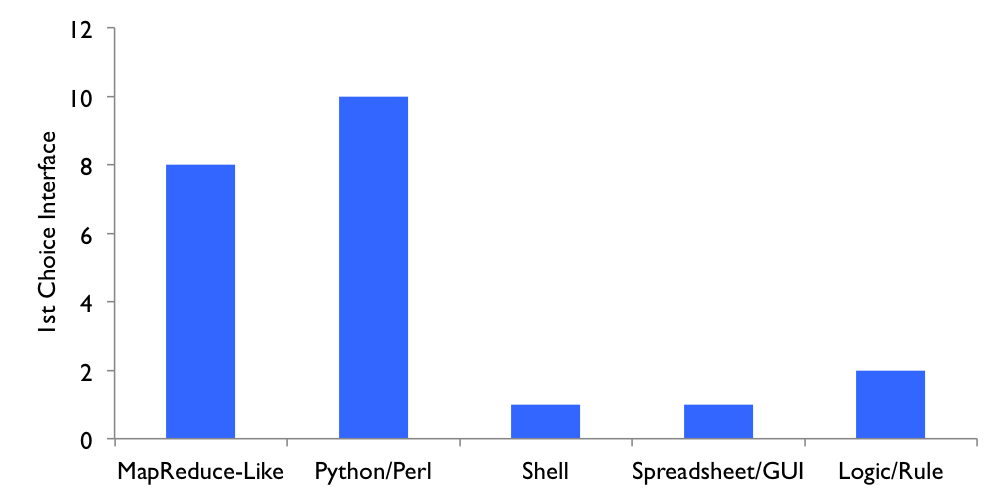
\includegraphics[width=\columnwidth]{datafigs/hilda-interface.png}
 \caption{Top ranked responses to: ``Which of the following tools/interfaces/languages do data scientists at your organization prefer for manipulating data, including extraction, schema transformations, and outlier removal, to make analysis easier or more reliable. Please Rank.''\label{fig:interfaces}}
\end{figure}


\subsection{Themes}\label{sec:themes}
We highlight several of the themes we discovered from the survey and the interviews: (1) the tension between infrastructure engineers and data analysts, (2) debugging and validation in data cleaning, and (3) methodology and over-fitting.

\subsubsection{Analysts vs. Infrastructure}
As noted by our demographics analysis, there are three main segments of data engineers: analysts, infrastructure engineers, and those who do both.
One of the most important themes that we discovered in the data was the divide between infrastructure engineers and analysts in how these groups address data quality problems. In particular, we see a difference in the way that these two groups of participants conceptualize dirty data, the solutions, and repair procedures.

One of the most significant tensions between the infrastructure engineers and analysts is about the definition of dirty data. While the infrastructure engineers are in charge of the data ingest pipelines, ETL, and other pre-processing steps, it is often the analysts who get to ``define'' what is dirty. One infrastructure engineer noted the frustration about being caught in the middle between the business units that generated the data and the analysts querying the data:

\vspace{0.5em}
\emph{There are often long back and forths with senior data scientists, devs, and the business units that provided the data on data quality. It is almost never a smooth process. The vast majority of problems are in turning semi-structured data into features. What placeholder value is sensible to use for a missing value, do we replace it with the mean or nearest neighbor; or is a variable ordinal or categorical? These are tough questions that often can only be answered by the business unit themselves. We try to get them to do some of this work but it inevitably falls on us esp. if it is a big unit.}

\vspace{0.5em}

The tension between the infrastructure engineers and the data analysts seems to stem from the semantics of data and who knows these semantics. Our responses also suggest that the definition of data error is highly analysis dependent. In response to how she defines dirty data, one analyst responded,

\vspace{0.5em}
\emph{Domain expertise, I guess. I wish there were a more rigorous way to do this but we look at the models and guess if the data are correct. -Analyst}

\vspace{0.5em}

This is in contrast to how infrastructure engineers want to handle data quality problems. 
Several infrastructure engineers noted that they saw dirty data as symptomatic of an error in the processing pipeline (i.e., a software bug or incorrect schema). Their goal was to rectify the bug or drop the corrupted data with a minimal impact on system SLOs:

\vspace{0.5em}
\emph{There are software bugs in the application such as edge cases that are not handled or changes to the services by programmers that have unintended consequences. Fixing data errors in a high-availability setting is challenge as it may require shutting of services. -Infrastructure Engineer}

\vspace{0.5em}

Most of the infrastructure engineers surveyed used sampling or unit testing to detect obvious problems in the data processing pipeline, for example,

\vspace{0.5em}
\emph{We have checks for file consistency, if the end of files look like the write was interrupted early, whether the size of a file seems significantly bigger or smaller than usual, etc. we check data with some standard queries to make sure the files have the expected range of values, ie for every country, and every minute of the day there was data. -Infrastructure Engineer}

\vspace{0.5em}

Such approaches require a clear definition of dirty data that is independent of the downstream analysis. Even worse, one consultant from a large database vendor noted that errors might be found well after some result is reported:

\vspace{0.5em}
\emph{Most of these errors are subtle enough that the analysis will go through e.g., with standard null value semantics of SQL, but give an incorrect answer. Usually is only caught weeks later after someone notices something like...well the Wilmington branch cannot have 1M sales in a week}




  

How do we detect dirty data?

How do we deal with dirty data?: 

Is Dirty Data Too Big?: To both groups of participants we asked the question “Has the scale of the data ever made it challenging to clean”. (k/N) We found that most of the self-reported infrastructure engineers suggested that scale was NOT an issue, while we found that (k/N) the reverse was true among the data analysts. This suggests that the type of dirty data is important to the question of scale. Errors that are semantic in nature may be harder to clean and detect as they require more discretion from the analysis.

“Build around common formats, otherwise it's all domain- and content-specific. Without fail, a non-trivial effort is required to "reduce problem to one previously solved", whether it be data access or translation of format for use with pre-existing tools.”-Infrastructure Engineer

“We usually do not do rigorous validation of data cleaning. We typically clean our data until the desired analytics works without error. This is not desirable but practical since in most cases data error is probably overshadowed by errors/inaccuracies in the models themselves.” -Data Analyst

.

Iteration vs. Interactiveness

“Do your level best on initial sample of data, determine what are exceptions and build filters. Iterate with greater knowledge.”

“Iterative process, where I assess biggest problem, devise a fix, re-evaluate. It is dirty work.”

“Usually the most time is spent getting the data into a state where your code even runs. After that, we make sure that we can explain every trend seen in the analysis.”

Semantics of the data and who knows it

“Domain expertise, I guess. I wish there were a more rigorous way to do this but we look at the models and guess if the data are correct.”

“When records are dirty, we usually identify the source of truth (in our case a hospital) and call them and figure out what is going on.”

“Much of the data cleaning and formatting logic goes into design views of the data that exclude errors or particularly questionable data. We design such processed data views with the help of development operations. Of course there are times when we have to go back to the source data to figure out if there are any artifacts in our analysis.”





Interactive vs noninteractive

How does debugging/validating correct cleaning get done?

The 99 percent

Overfitting the cleaning

\section{The Future of Data Cleaning}\label{sec:future}
Here’s a general system/interactive loop that is pie in the sky that would work for the 99\% cases

Concrete Technical Problems 1 2 3 4 with possible solutions.

Usability -- mapping user interactions to the many many algorithms

Automate what you can -- string value data cleaning.  Wha??  What has been automated and what we think can be automated aka hyperparameter tuning. 

What effects did this cleaning have on the whole dataset?

Debugging for data cleaning

Combating overfitting


Future directions for interactive data cleaning/integration

* Here’s a general system/interactive loop that is pie in the sky that would workfor the 99% cases.
    * Data cleaning is user and context dependent.  So much relies on the developer’s, or downstream user's expert knowledge that interactive solutions are needed.    
    * In fact, in some cases, the data cleaning process is divorced from the users using the data cleaning, which is surprising given the context-sensitive nature.
    * trying cleaning procedures, algorithms, tuning parameters out, and evaluating the results through visual inspection of computed metrics, or the cleaned data
    * Needs highly interactive systems, and often visual systems for domain experts
    * Figure 1 shows a highlevel loop
    * Only when combined into a single system does it make sense
    * This motivates a set of interesting technical problems that we outline below.
* A language or languages for data cleaning.  An operation, such as deduplication involves a large number of possible algorithms or sytems techinques, ranging from crowdsourced solsutions(REF Anhai), machine learning-based fuzzy matching(REF).  It is often easier for a user to provide correct results rather than.
* Be careful about survey biased towards technical people, not those that use GUIs. 
* Usability: Tied with the language are a set of interactions to match the language operations (REF joe’s CIDR paper).  This is admittedly an amorpheous topic.  (REF agreementmaker work)
* Goal oriented cleaning.  General data cleaning is rarely needed, and pay-as-you-go solutions(REF data spaces) are needed in most applications.   This begs the qusetion for hminimizing expert involvement.   Solutions such as sampleclean are oriented towards specializing the human effort towards porudictive tasks that maximize the cleaning for a particular application.  
* Automation. 
    * Hyperparameter tuning, however visual inspection by manually tuning each or combinations of parameters is both slow and and error-prone.  Automated hyperparemeter tuning (REF evan)
    * String value munging, either deduplication, extraction, fixes.  Existing tools are often not sufficient and user intervention (REF Wrangler) is necessary.  However even in this settings, ways to generate suggestions and show them is better than users picking operations to perform.
    * active learning is used, but only for crowd workers that fit inside an operator good progress folks.
    * Opporutinity let the expert be the human in the loop.  The data analyst IS the human in the loop.
    * Let humans do what they do best, machines to the rest.
* Testing and debugging cleaning.  Data cleaning does not live within a vacuum.  It is often motivated by a set of desired applications, and .  How can it be tested?  For example, what effects will introducing or modiying a data cleaning procedure have on the rest of the dataset, or the downstream application?  For example, in our survey several respondents noted that their evaluation was based on whether the downstream applicaiton compiles or not.
    * Reference Self eval idea.  long pipeline from cleaning and output, so insert inspection.  
    * Reference benchmarking work and systematic ways to evaluate the efficacy of an approach when there is ground truth and when there is no ground truth.
* (SANJAY) Overfitting and sharing.   It is easy to overfit the data cleaning to the intricacies of a particular application and the data for that application.  Although this is easy to do, it makes it difficult to share and re-use data cleaning procedures for similar tasks in the future, or share within an organization.  In these cases, tools to help prevent overfitting, similar to regularization in machine learning, are needed to help generalize data cleaning workflows into reusable components.  High level scripting languages can help in this regard, but automated tools are also needed.

In summary, we are in the early days of highly interactive data cleaning and preparation and we are optimistic about the improvement that can be made by bringing user interactivity into the process.
lo


\bibliographystyle{abbrv}
\bibliography{ref} 
\clearpage
\normalsize \selectfont

\end{document}

